\graphicspath{ {./content/results/figures/} }

\section{Results}
\label{sec:res}

\subsection{Qualitative}

\begin{figure}
  \centering
  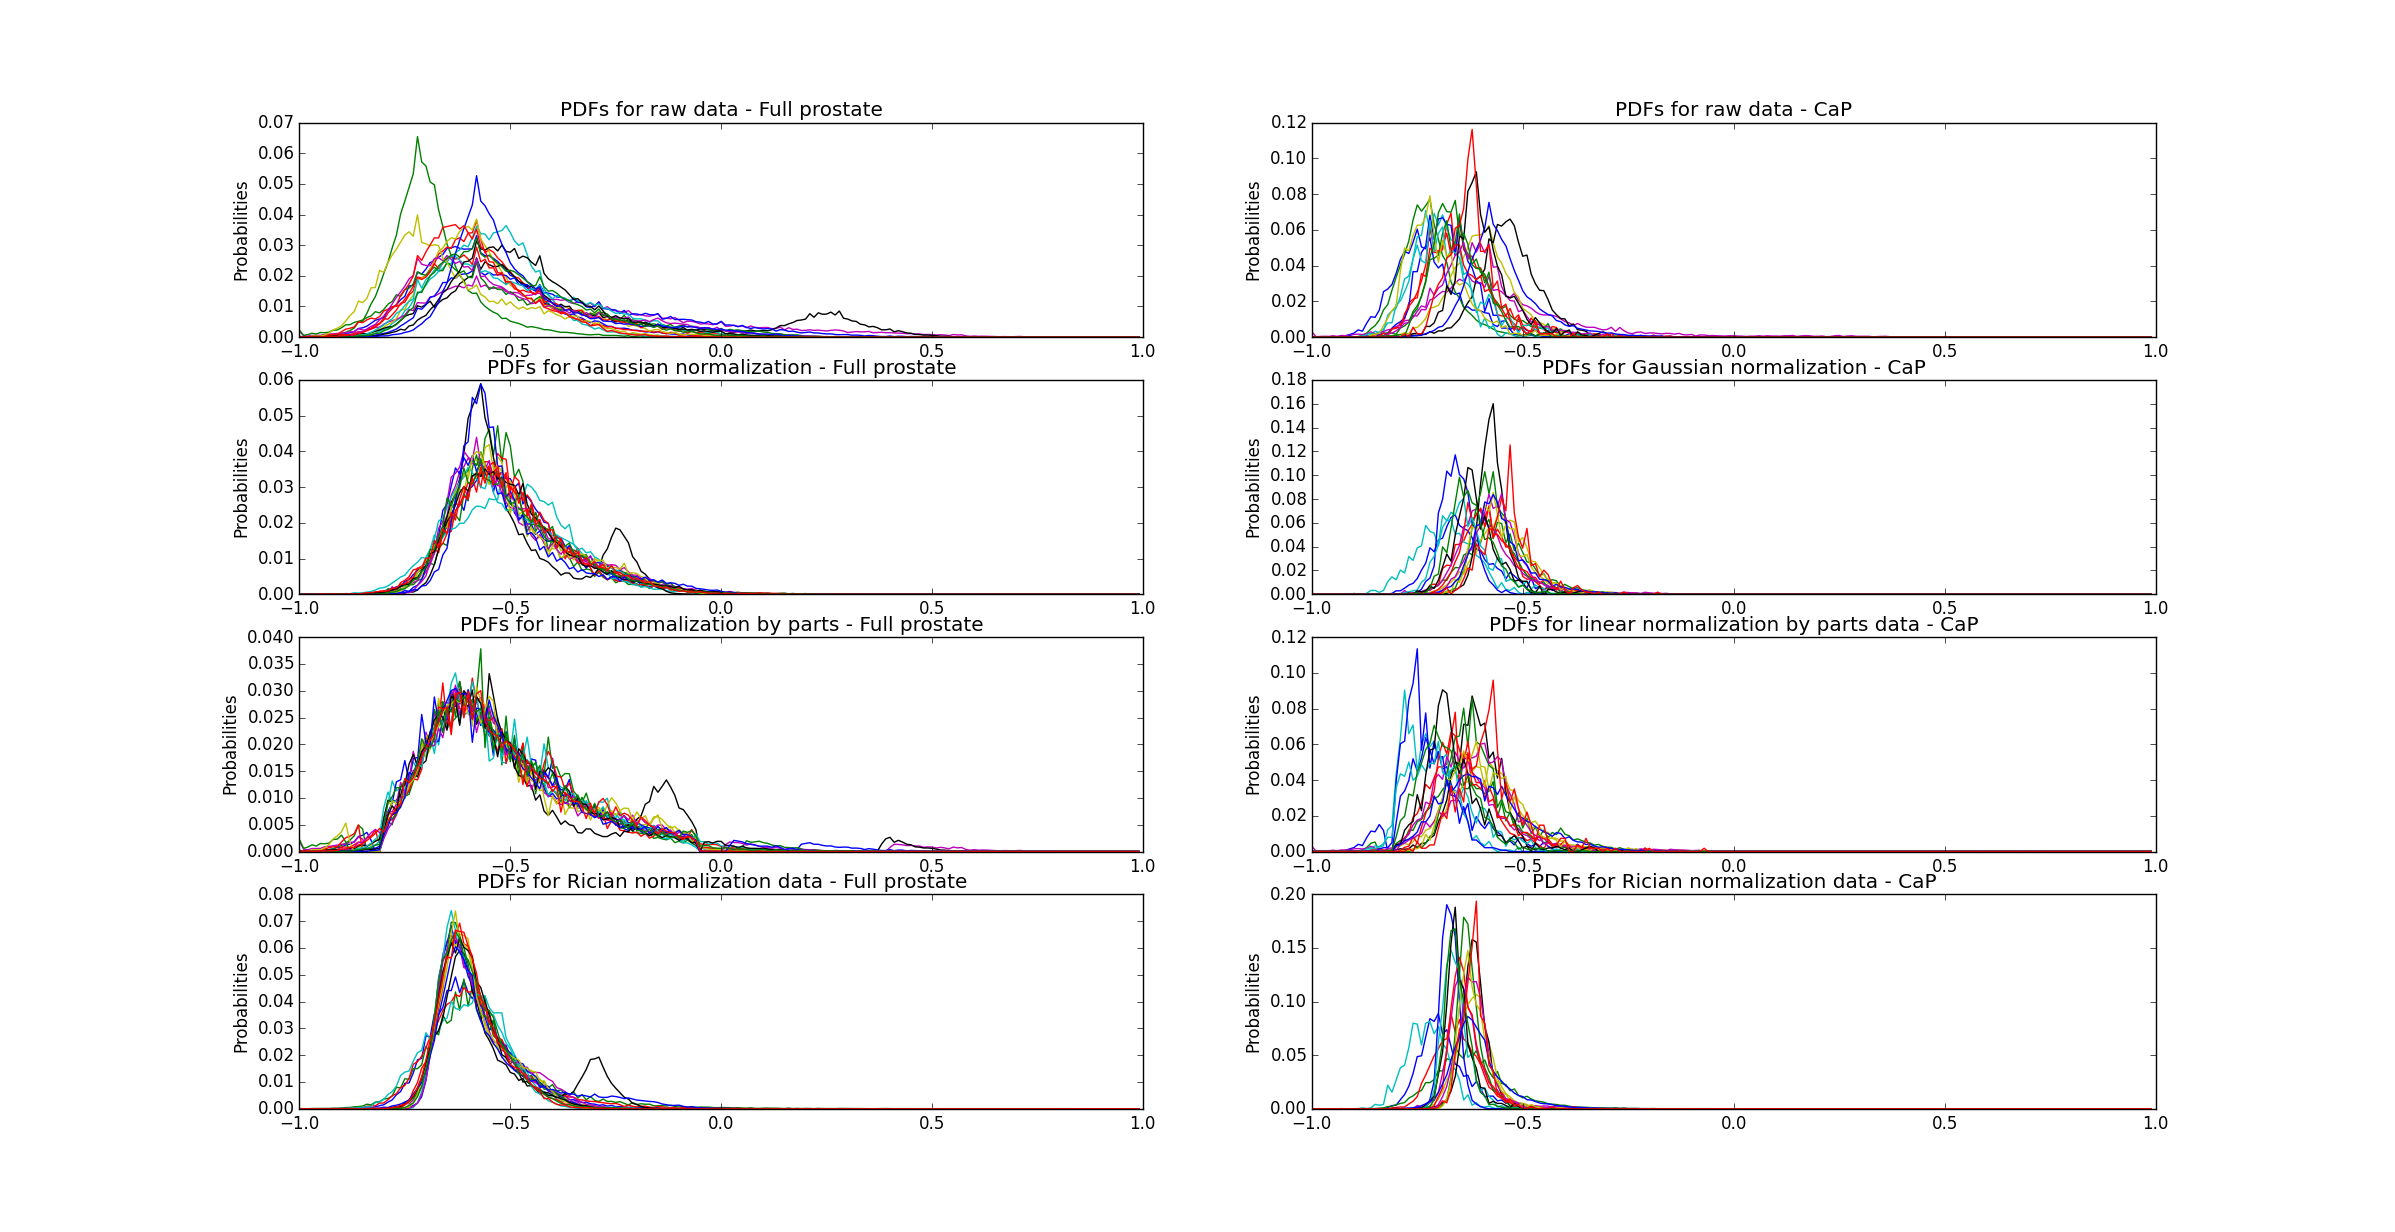
\includegraphics[width=0.8\textwidth]{qualitative.png}
  \caption{Qualitative evaluation by visual inspection of the alignment of the \ac{pdf}s for the full prostate and the \ac{cap}.}
  \label{fig:qu}
\end{figure}



\subsection{Quantitative}

\begin{figure*}
  \centering
  \subfloat[][]{
    \label{fig:qtfull}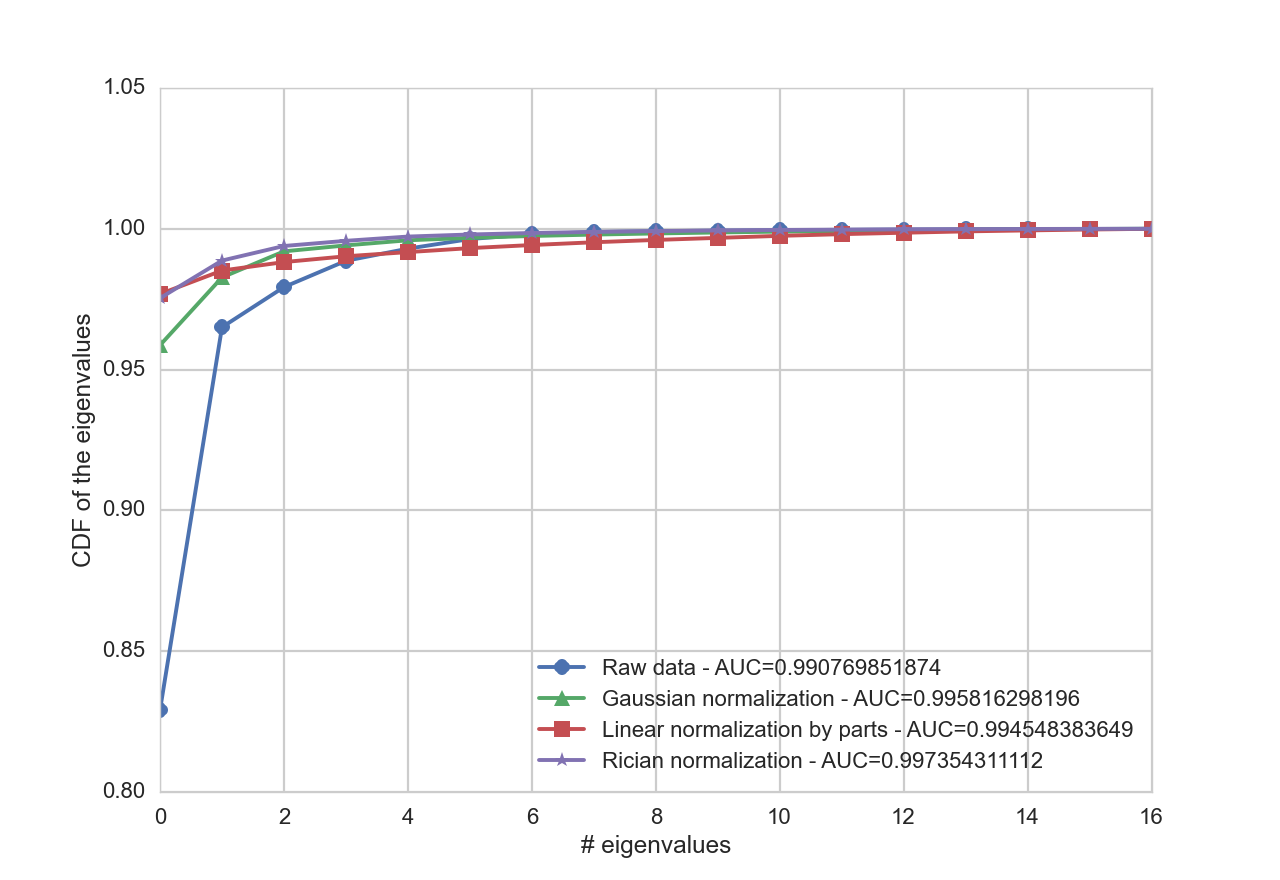
\includegraphics[width=0.45\textwidth]{quantitative_1.png}}\hfill
  \subfloat[][]{
    \label{fig:qtcap}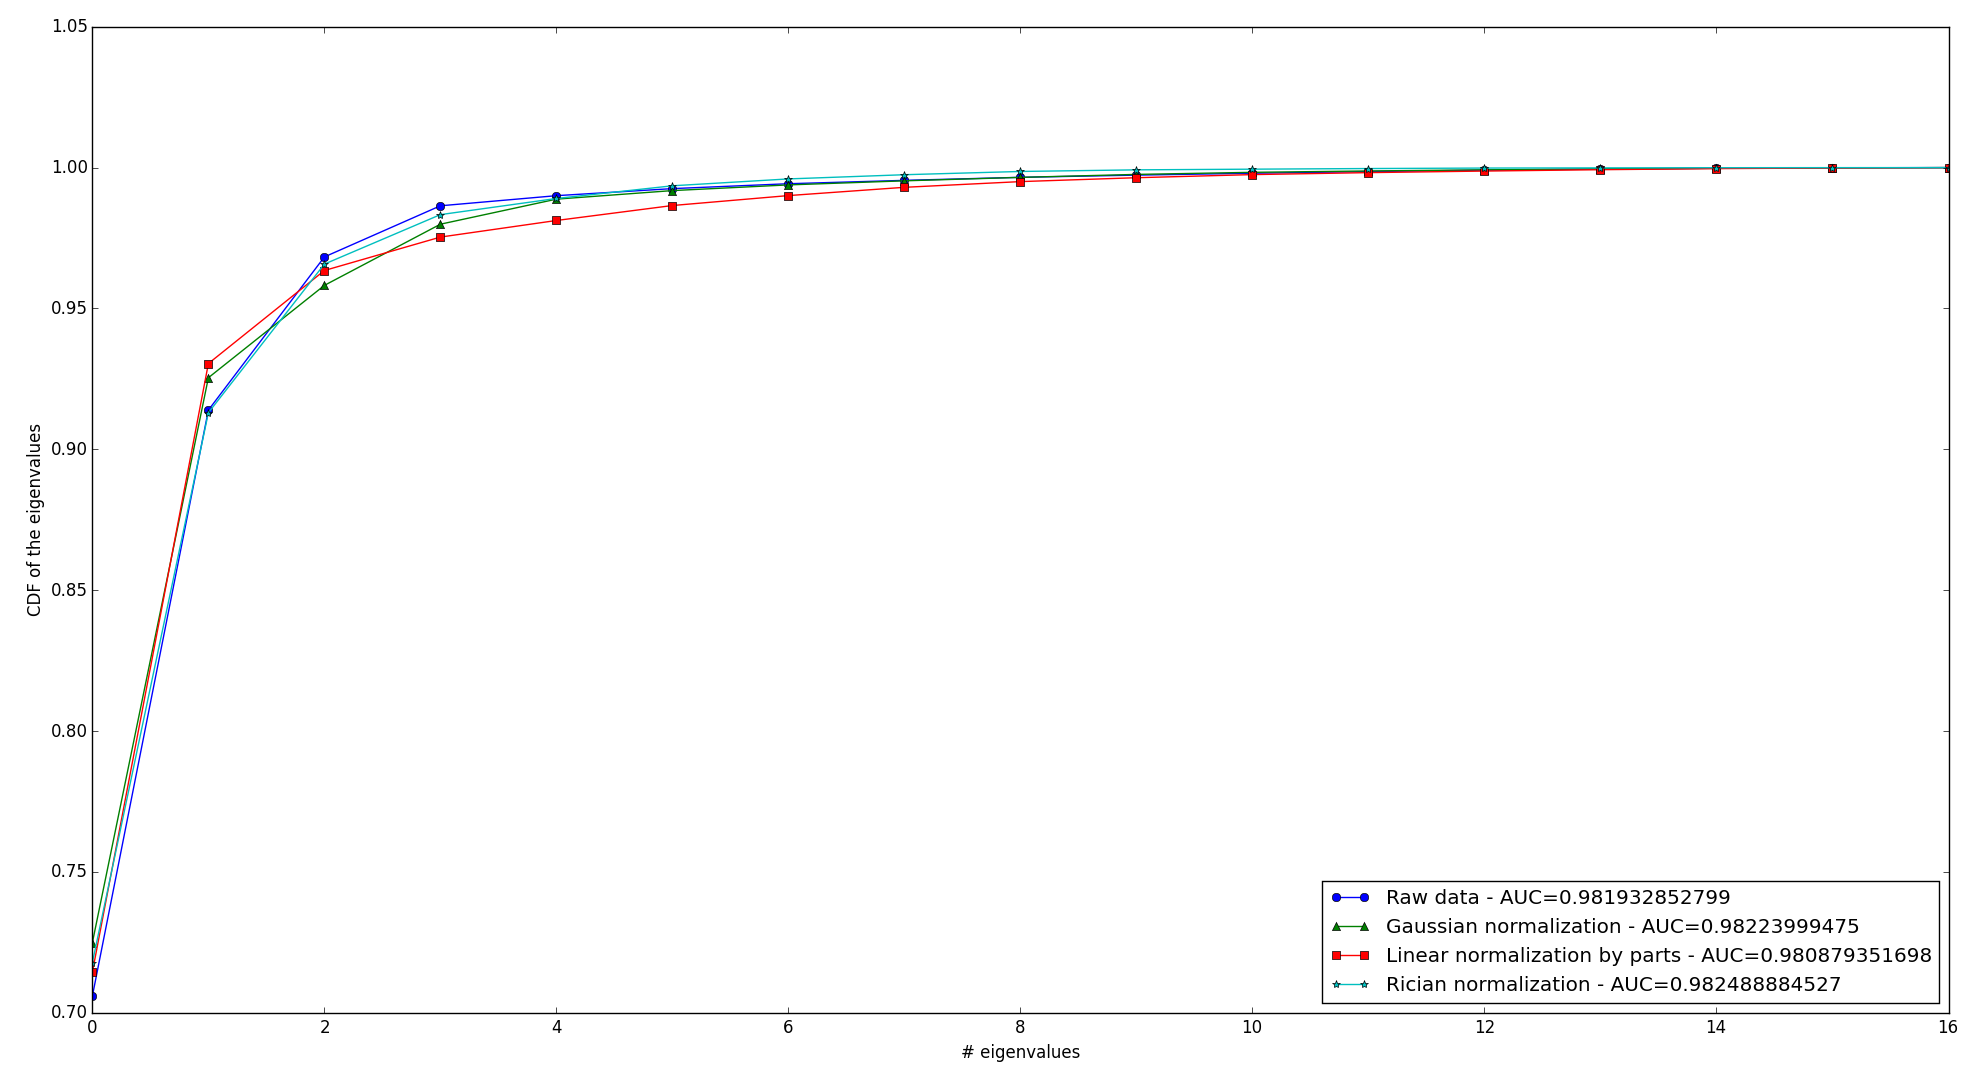
\includegraphics[width=0.45\textwidth]{quantitative_2.png}}
  \caption{Spectral evaluation using \ac{pca} decomposition: \protect\subref{fig:qtfull} evaluation considering the full prostate, \protect\subref{fig:qtcap} evaluation considering only the \ac{cap}.}
  \label{fig:qt}
\end{figure*}

%%% Local Variables: 
%%% mode: latex
%%% TeX-master: "../../master"
%%% End: 
